
%(BEGIN_QUESTION)
% Copyright 2010, Tony R. Kuphaldt, released under the Creative Commons Attribution License (v 1.0)
% This means you may do almost anything with this work of mine, so long as you give me proper credit

Examine this P\&ID for a level control system in a vessel where two different fluids (Feed A and Feed B) are mixed together.  The level control valve (LV) is air-to-close (fail-open):

$$\includegraphics[width=15.5cm]{i01836x01.eps}$$

Determine the effect on the control system's regulation of liquid level inside the vessel if Feed A suddenly stops but the flow of Feed B continues at its normal rate.  Assume all loop components are properly configured, that the controller is well-tuned, and that a significant amount of time has passed since Feed A stopped.  Compare these conditions with what they were before the process change:

\begin{itemize}
\item{} Liquid level will: {\it increase} from what it was before, {\it decrease} from what it was before, or {\it remain the same} as before
\vskip 10pt
\item{} Control valve will: {\it open up} further, {\it close down} more, or {\it remain in the same position} 
\end{itemize}

\underbar{file i01836}
%(END_QUESTION)





%(BEGIN_ANSWER)

\begin{itemize}
\item{} Liquid level will: {\bf remain the same as before}  
\vskip 5pt
\item{} Control valve will have: {\bf close down more}
\end{itemize}

%(END_ANSWER)





%(BEGIN_NOTES)

{\bf This question is intended for exams only and not worksheets!}.

%(END_NOTES)


